\chapter{Primitive Network Completion}

In this chapter we discuss the idea of network completion and demonstrate a relatively brute-force method of using a segmentation result to solve some of the network completion problem.

One of the biggest shortcomings of our demonstrated segmentation methods is that they frequently result in gaps in parts of the network. We demonstrate a way to rectify this problem in certain situations, and then discuss how to extend these arguments to fill larger, more uncertain gaps.

First, once we've produced a segmentation, we thin it down with \cite{thinning} and look for endpoints of an otherwise connected point. Using a $3\times 3$ structuring element, we iterate over each pixel and identify how many local neighbors it has. If a pixel has zero or one local neigbors, we identify it as an endpoint of the partial network. After identifying these endpoints, we assign each a label $(i,j)$ depending on where the neighboring pixel is located, as according to \cref{fig:endpoint_labels}. We deem two endpoints potentially connectible only if they're not connected on the same side. That is, their labels $(i,j)$ and $(i',j')$ must have $i\ne i'$ or $j\ne j'$ (unless $i$ or $j$ is 1). For example, if an endpoint is connected to the partial network on its top side, any endpoint that connects to it cannot also be connected to a network on its top. If a pixel has no connections at all, with label $(1,1)$, we do not restrict its connetions at all. To save time (though we don't anticipate it will affect the result much), we also restrict pais from being more than a set distance away (in this case, 100 pixels in Euclidean length).

\begin{figure}
	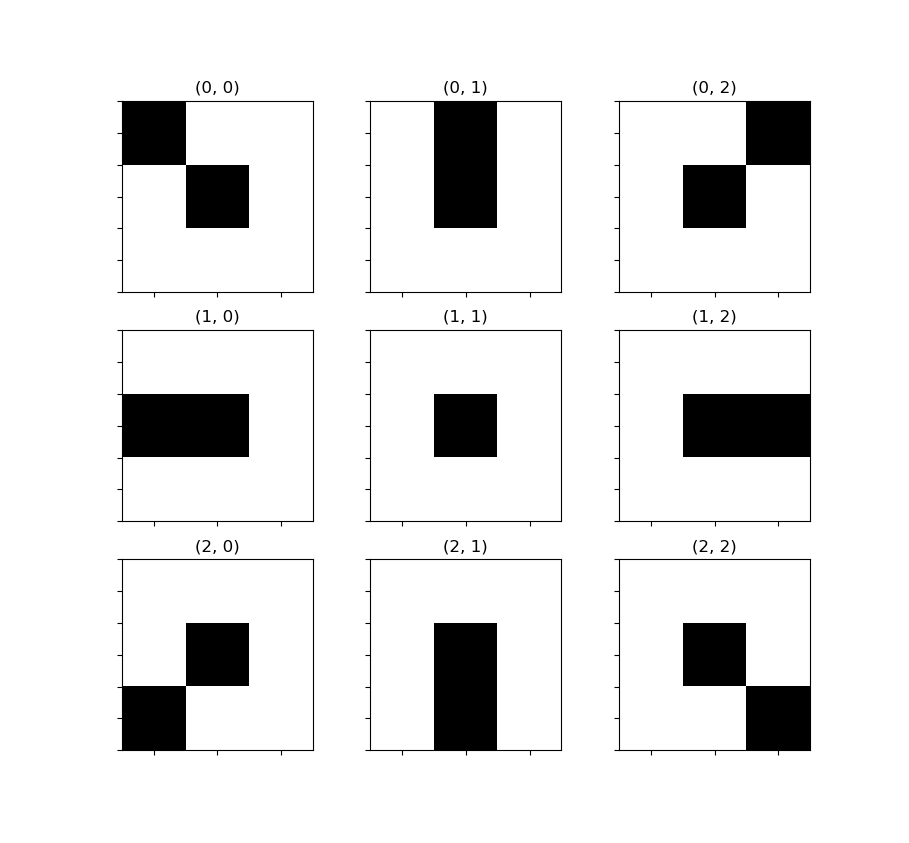
\includegraphics[width=.85\textwidth]{endpoint_labels}
	\caption{Endpoints labels based on adjacent neighbor location}
	\label{fig:endpoint_labels}
\end{figure}

After we limit the connections, we consider each pair of endpoints and draw a straight line segment between the two. If that passes through a point where $\Vmax$ is 0, we disallow that pair as well. We also disallow any line which crosses any part of the network which is known to exist.
Finally, from the list of all remaining pairs of endpoints, we simply select the path along which the maximum mean value of $\Vmax$ is achieved. \cref{fig:network-completion-all-pairs} shows non-violating paths between end-point pairs, and \cref{fig:network-completion} shows a partially completed network (in yellow) overlaid on $\Vmax$.



\begin{figure}
	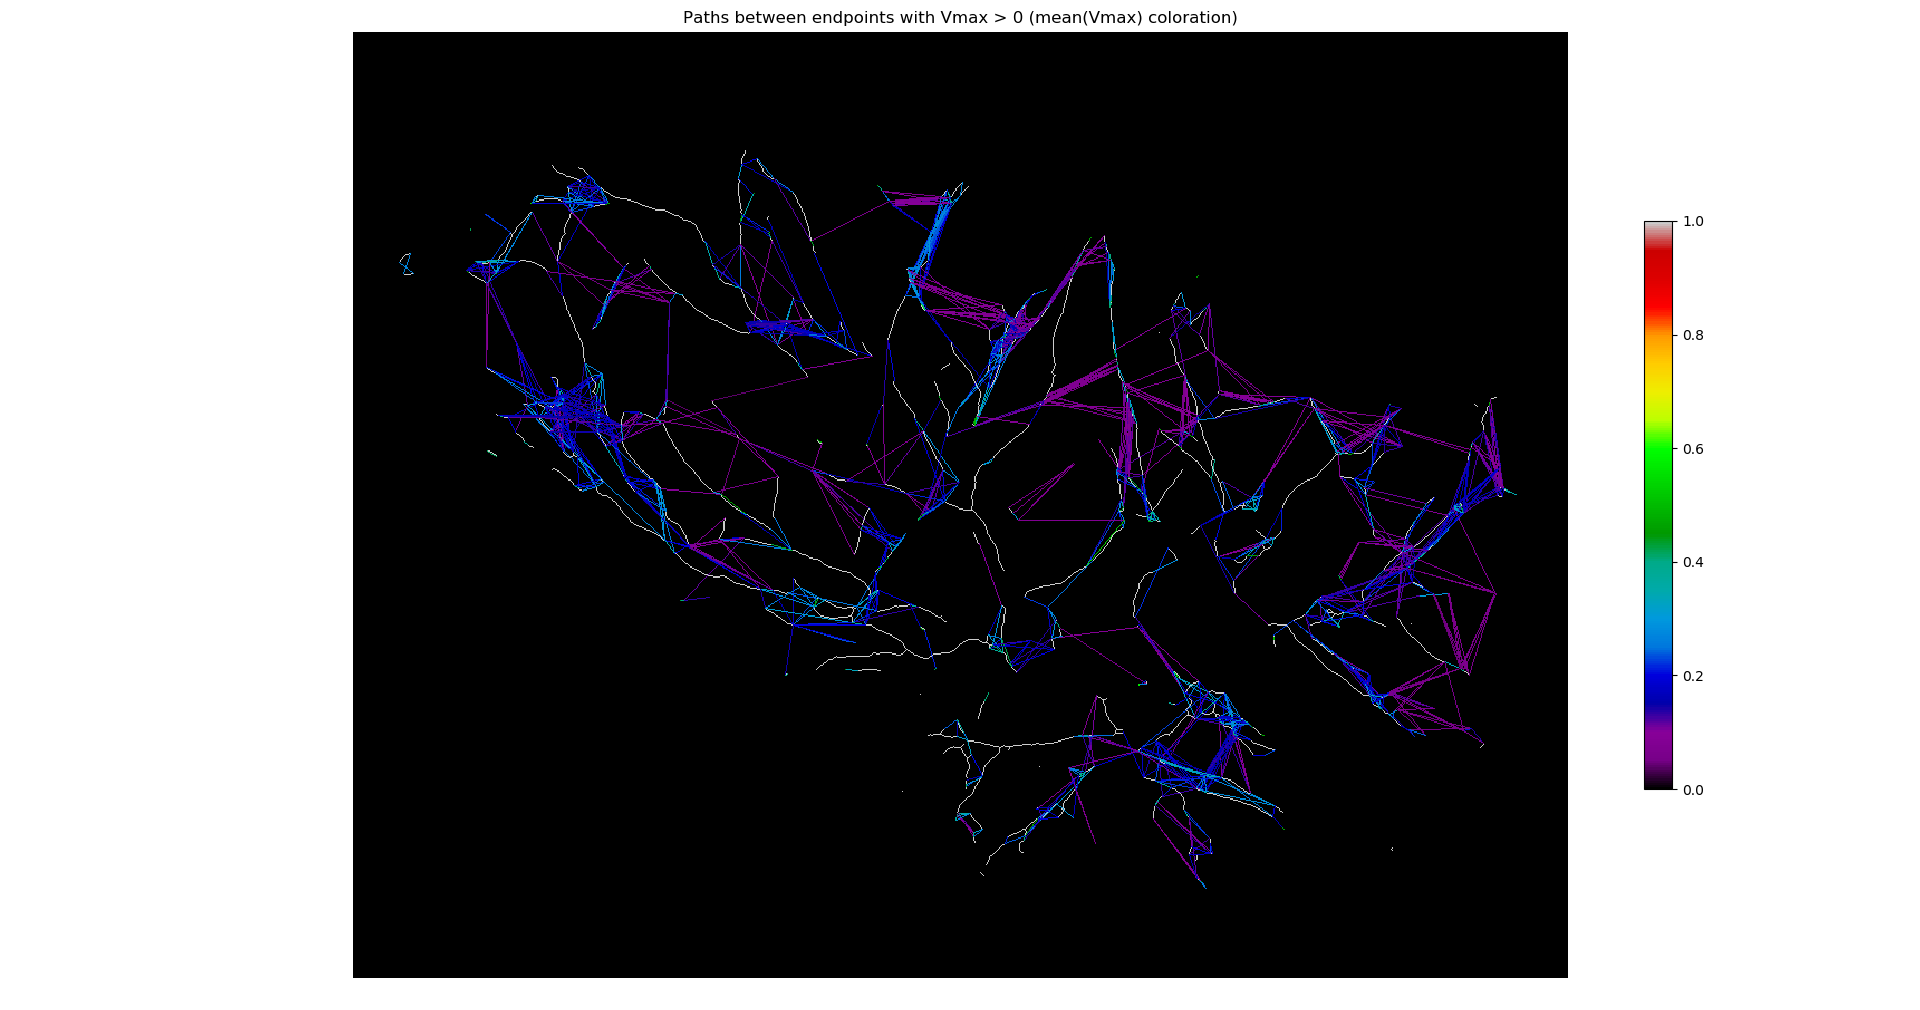
\includegraphics[width=\linewidth]{paths_between_endpoints_positive_score}
	\caption{All lines between endpoints with nonzero $\Vmax$}
	\label{fig:network-completion-all-pairs}
\end{figure}
\begin{figure}
	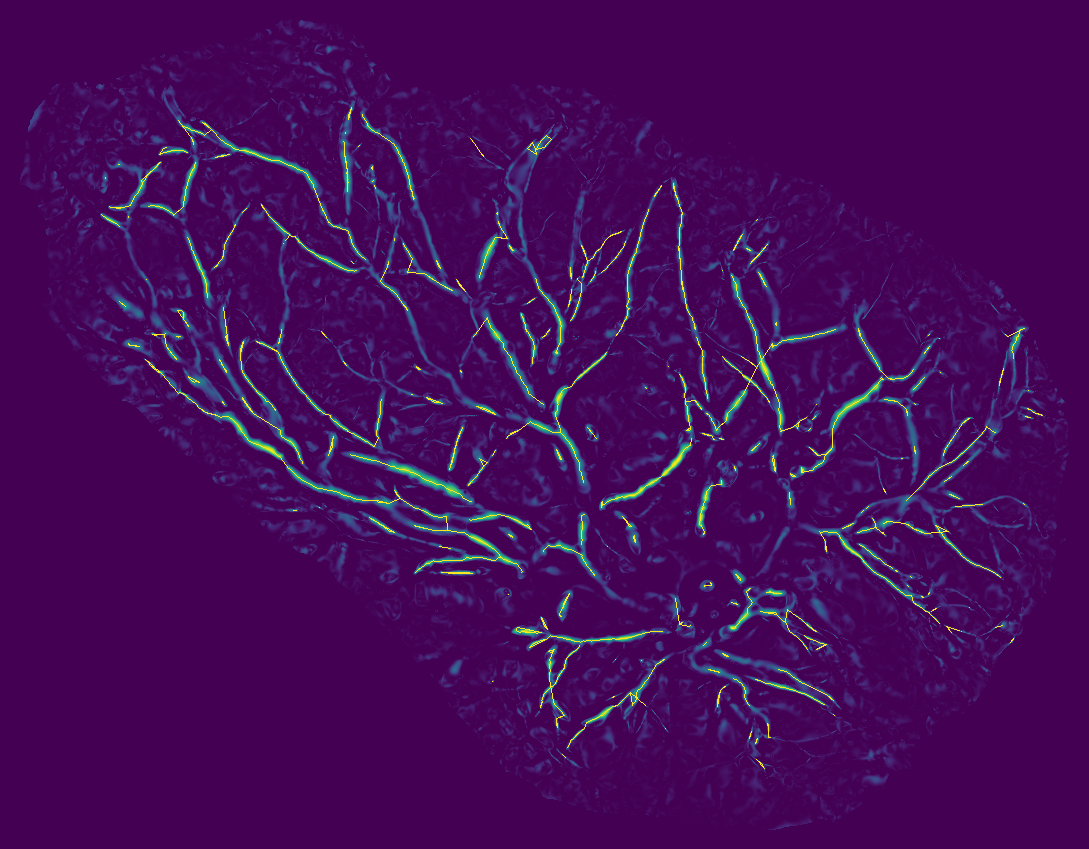
\includegraphics[width=\linewidth]{completed_by_nearest_to_line_mash}
	\caption{Partially completed network}
	\label{fig:network-completion-end-result}
\end{figure}

We show the complete process for comparison on two different samples. 

\begin{figure}
	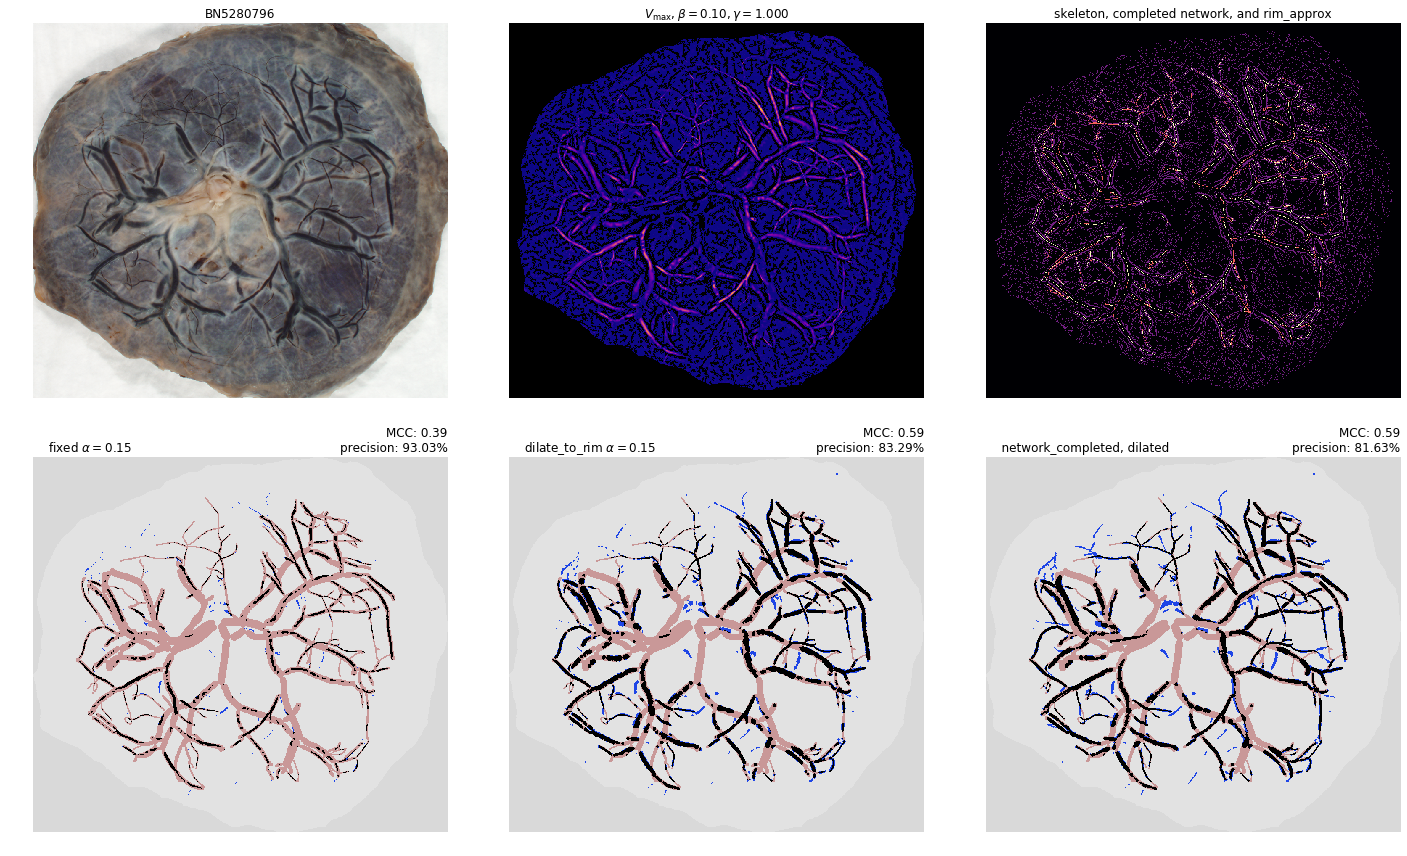
\includegraphics[width=\linewidth]{sample_network_completion}
	\caption{Trough Dilation and Network Completion (Example 1)}
	\label{fig:network-completion-demo-1}
\end{figure}
\begin{figure}
	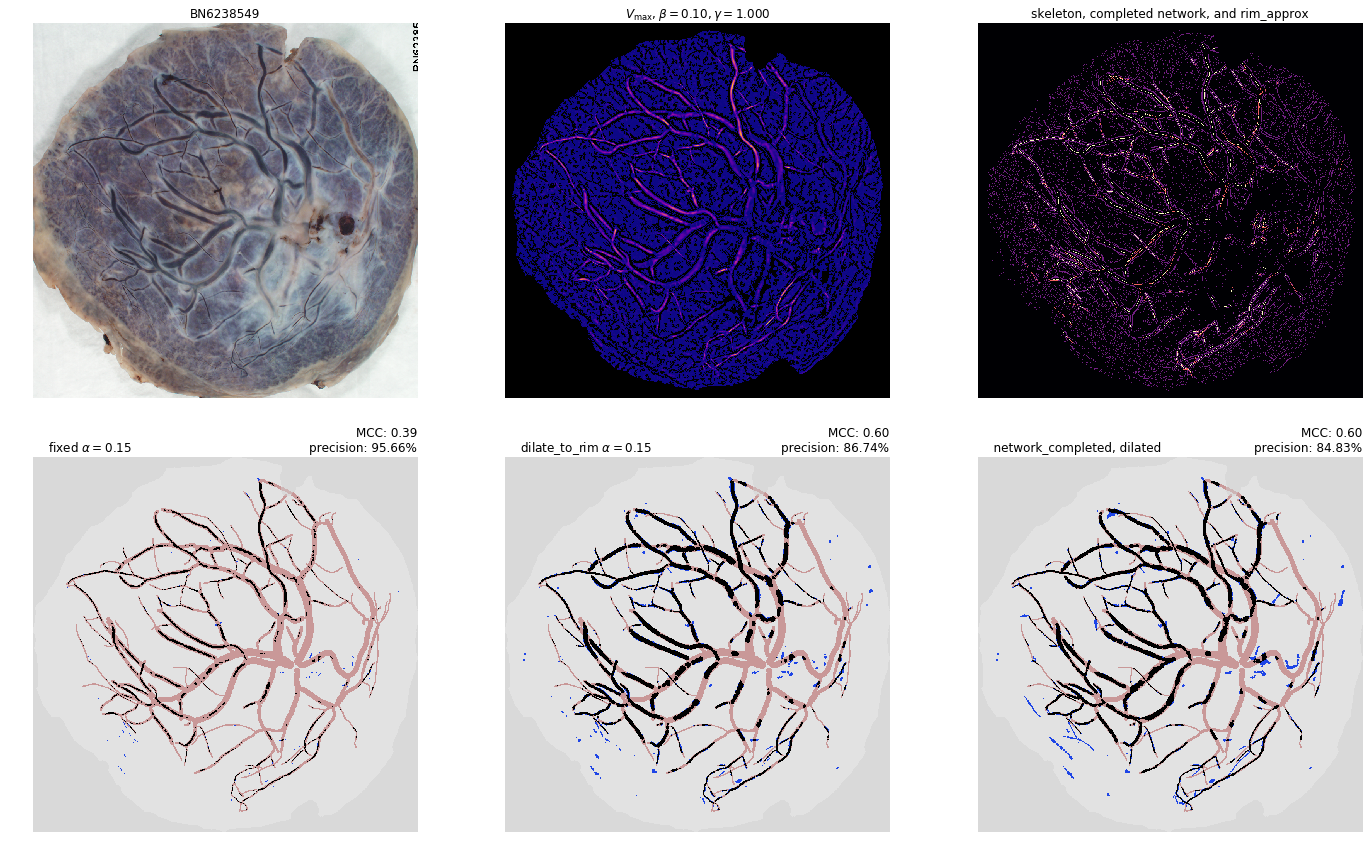
\includegraphics[width=\linewidth]{sample_network_completion_2}
	\caption{Trough Dilation and Network Completion (Example 2)}
	\label{fig:network-completion-demo-2}
\end{figure}


